\documentclass[../distribution_theory_notes.tex]{subfiles}
\begin{document}
\section{Aula 24 - 18 de Novembro, 2024}
\subsection{Motivações}
\begin{itemize}
	\item Continuação das propriedades da convolução de duas distribuições;
	\item Existência e unicidade de soluções por meio de uma solução fundamental;
	\item Regularidade das soluções e operadores hipoelípticos.
\end{itemize}

\subsection{Apêndice: Continuação das Propriedades da Convolução \(u_{1}*u_{2}\)}
Retomemos as propriedades da convolução de duas distribuições quando ao menos uma delas possui suporte compacto.

\medskip
\noindent\textbf{(I)} \(\delta\in\mathcal{E}'\) é o \textbf{elemento neutro} da convolução:
\[
	\delta*u=u*\delta=u,
	\qquad \forall u\in\mathcal{D}'.
\]

\medskip
\noindent\textbf{(II)} A convolução é \textbf{associativa}:
\[
	u_{1}*(u_{2}*u_{3})=(u_{1}*u_{2})*u_{3},
\]
se ao menos dois fatores tiverem suporte compacto. Em particular, \(*\) é uma operação interna em \(\mathcal{E}'\), e faz sentido tomar as potências
\[
	u^{k}\coloneqq \underbrace{u*u*\cdots*u}_{k\text{ fatores}},
	\qquad \forall u\in\mathcal{E}',
\]
e considerar a série
\[
	\sum_{k=0}^{\infty}\frac{u^{k}}{k!},
\]
e indagar sobre sua convergência em \(\mathcal{D}'\), como uma espécie de ``\(e^{u}\)''.

\medskip
\noindent\textbf{(III)} Vale também a \textbf{comutatividade}:
\[
	u_{1}*u_{2}=u_{2}*u_{1}.
\]

\medskip
\noindent\textbf{(IV)} A derivação se torna um \textbf{operador do tipo convolução}, isto é,
\[
	\partial^{\alpha}(u_{1}*u_{2})
	=(\partial^{\alpha}u_{1})*u_{2}
	=u_{1}*(\partial^{\alpha}u_{2}).
\]
Assim,
\[
	\partial^{\alpha}u
	=\partial^{\alpha}(\delta*u)
	=(\partial^{\alpha}\delta)*u,
\]
e, portanto,
\[
	P(D)u=(P(D)\delta)*u.
\]

\medskip
\noindent\textbf{(V)} O suporte da convolução se localiza a partir dos suportes dos fatores:
\[
	\mathrm{supp}(u_{1}*u_{2})
	\subseteq \mathrm{supp}(u_{1})+\mathrm{supp}(u_{2}).
\]
Isto pode ser provado a partir do seguinte lema.

\begin{lemma*}
	Se
	\[
		u_{j}\stackrel{*}{\longrightarrow}u,
		\qquad \mathrm{supp}(u_{j})\subseteq F_{j},
	\]
	em que \((F_{j})\) é uma sequência de fechados com \(F_{j}\supseteq F_{j+1}\), então
	\[
		\mathrm{supp}(u)\subseteq F
		\coloneqq\bigcap_{j=1}^{\infty}F_{j}.
	\]
\end{lemma*}

\medskip
\noindent\textbf{(VI)} Em \(u_{1}*u_{2}\), se \(u_{1}\in\mathcal{C}^{\infty}\), ou \(u_{2}\in\mathcal{C}_{c}^{\infty}\), as definições nova e antiga coincidem.

\subsection{Existência e Unicidade de Soluções}
Tendo agora definido a convolução \(u_{1}*u_{2}\) de duas distribuições com uma delas possuindo suporte compacto, e estabelecido as suas ``propriedades operacionais'', vejamos como elas podem ser úteis no estudo das propriedades das soluções de uma EDP não-homogênea
\[
	P(D)u=v,
\]
no caso em que \(P(D)\) é um ODPCC possuindo solução fundamental \(E\), ou apenas uma ``parametrix''.

\begin{def*}
	Dizemos que \(P(x,D)\) é \textbf{localmente resolúvel} em \(\Omega\) quando todo \(x_{0}\in\Omega\) possui uma vizinhança \(U\ni x_{0}\) tal que, para toda \(f\in\mathcal{C}_{c}^{\infty}(U)\), existe \(u\in\mathcal{D}'(U)\) com
	\[
		P(x,D)u=f.\qquad \square
	\]
\end{def*}

No caso em que uma das distribuições possui suporte compacto, a aplicação
\[
	\mathcal{D}'\times\mathcal{E}'\longrightarrow\mathcal{D}',
	\qquad (u,v)\longmapsto u*v,
\]
é bilinear.

\noindent\textbf{\underline{Existência}:} Se \(v\in\mathcal{E}'(\mathbb{R}^{n})\), então
\[
	u\coloneqq E*v
\]
é solução de \(P(D)u=v\). Com efeito,
\begin{align*}
	P(D)u
	 & =\sum_{|\alpha|\leq m}a_{\alpha}(\partial^{\alpha}E)*v            \\
	 & =\left(\sum_{|\alpha|\leq m}a_{\alpha}\partial^{\alpha}E\right)*v
	=\delta*v=v.
\end{align*}
Observamos apenas que \(u=E*v\) está bem definida porque \(v\in\mathcal{E}'\), de modo que as propriedades anteriores podem ser aplicadas. Em particular,
\[
	v\in\mathcal{C}_{c}^{\infty}
	\quad\Longrightarrow\quad
	u=E*v\in\mathcal{C}^{\infty}.
\]

\noindent\textbf{\underline{Unicidade}:} Seja \(v\in\mathcal{E}'\). Se \(u\in\mathcal{E}'\) resolve
\[
	P(D)u=v,
\]
então \(u=E*v\). Realmente, pois, sendo \(u\in\mathcal{E}'\), vale
\[
	P(D)(E*u)=E*(P(D)u),
\]
donde podemos escrever
\[
	u=\delta*u=(P(D)E)*u=E*(P(D)u)=E*v,
\]
estabelecendo a unicidade de solução com suporte compacto de \(P(D)u=v\).

\begin{tcolorbox}[
		skin=enhanced,
		title=Observação,
		fonttitle=\bfseries,
		colframe=black,
		colbacktitle=cyan!75!white,
		colback=cyan!15,
		colbacklower=black,
		coltitle=black,
		drop fuzzy shadow,
	]
	Vale também a ``continuidade com relação aos dados iniciais'': se
	\[
		f_{j}\stackrel{j\to\infty}{\longrightarrow}f
		\quad\text{em }\mathcal{C}_{c}^{\infty},
	\]
	então
	\[
		u_{j}=E*f_{j}
		\stackrel{j\to\infty}{\longrightarrow}
		E*f=u
		\quad\text{em }\mathcal{C}^{\infty}.
	\]
	Ou seja, as soluções \(u_{j}\) estão próximas da solução \(u\) se os dados \(f_{j}\) estão próximos do dado \(f\).
\end{tcolorbox}

\subsection{Regularidade das Soluções}
Queremos estudar a regularidade local das soluções de uma equação
\[
	P(D)u=f
\]
em um aberto \(\Omega\subseteq\mathbb{R}^{n}\), no caso em que \(f\in\mathcal{C}^{\infty}\) numa vizinhança de um ponto \(x_{0}\in\Omega\), mas não necessariamente possui suporte compacto. O caso \(f\in\mathcal{C}_{c}^{\infty}\) já está dado no caso anterior de existência.

Para isso, apresentaremos um conceito geral extremamente importante no estudo das EDPs.

\begin{def*}
	Sejam \(\Omega\subseteq\mathbb{R}^{n}\) um aberto e
	\[
		P(x,D)=\sum_{|\alpha|\leq m}a_{\alpha}(x)\partial^{\alpha}
	\]
	um operador diferencial parcial com coeficientes \(\mathcal{C}^{\infty}\) em \(\Omega\). Dizemos que \(P(x,D)\) é \textbf{(localmente) hipoelíptico}, ou simplesmente \textbf{hipoelíptico}, em \(\Omega\), quando, para toda \(u\in\mathcal{D}'(\Omega)\), tem-se
	\[
		\mathrm{supp\,sing}\bigl(P(x,D)u\bigr)
		=\mathrm{supp\,sing}(u).\qquad \square
	\]
\end{def*}

\begin{tcolorbox}[
		skin=enhanced,
		title=Observação,
		fonttitle=\bfseries,
		colframe=black,
		colbacktitle=cyan!75!white,
		colback=cyan!15,
		colbacklower=black,
		coltitle=black,
		drop fuzzy shadow,
	]
	Para toda \(u\in\mathcal{D}'(\Omega)\) e todo \(P(x,D)\), vale sempre
	\[
		\mathrm{supp\,sing}\bigl(P(x,D)u\bigr)
		\subseteq \mathrm{supp\,sing}(u).
	\]
	Com efeito, se \(u\in\mathcal{C}^{\infty}(U)\), então
	\[
		\partial^{\alpha}u\in\mathcal{C}^{\infty}(U)
		\Longrightarrow
		a_{\alpha}(x)\partial^{\alpha}u\in\mathcal{C}^{\infty}(U)
		\Longrightarrow
		P(x,D)u\in\mathcal{C}^{\infty}(U).
	\]
	Logo, sendo \(V_{0} = \{x\in \Omega :\; \exists V_{x} \text{vizinhança de x}, P(x, D)u\in \mathcal{C}^{\infty}(U_{x})\}\)	, temos
	\[
		U\subseteq V_{0} \Rightarrow \mathrm{supp\,sing}(P(x, D)u) = \Omega \setminus{V_{0}}\subseteq \Omega \setminus{U}
	\]
	para todo U contido em \(V = \{x\in \Omega :\; \exists V_{x} \text{vizinhança de x}, P(x, D)u\in \mathcal{C}^{\infty}(U_{x})\}\); consequentemente,
	\[
		\mathrm{supp\,sing}(P(x, D)u)\subseteq \bigcap_{U\subseteq V}^{}\Omega \setminus{U}=\mathrm{supp}(u),
	\]
	Com isso, a definição significa que, a fim de que \(P(x, D)\) seja hiperbólico, devemos mostrar ``apenas'' que
	\[
		\mathrm{supp\, sing}(u)\subseteq \mathrm{supp\, sing}(P(x, d)), \quad \forall u\in \mathcal{D}'(\Omega),
	\]
	ou seja, em termos dos complementares, mostrar que
	\[
		\Omega\setminus{\mathrm{supp\, sing}(P(x, D)u)} \subseteq \Omega \setminus{\mathrm{supp\, sing}(u)}, \quad u\in \mathcal{D}'(\Omega ),
	\]
	isto é, se \(U\subseteq\Omega\) é aberto e
	\[
		P(x,D)u=f\in\mathcal{C}^{\infty}(U),
	\]
	então
	\[
		u\in\mathcal{C}^{\infty}(U).
	\]
	Em palavras, \(P(x,D)\) recupera, resgata, devolve ou determina a regularidade de \(u\) a partir da regularidade de sua imagem \(P(x,D)u=f\). Da mesma maneira, isso quer dizer que \(P(x,D)\) não transforma uma distribuição singular numa distribuição regular.
\end{tcolorbox}

\begin{example}
	\medskip
	\noindent\textbf{(1)} O operador
	\[
		P(D)=\frac{d}{dx}
	\]
	é hipoelíptico em \(\mathbb{R}\). De fato, se \(u\in\mathcal{D}'(\mathbb{R})\) é tal que
	\[
		\frac{du}{dx}=f\in\mathcal{C}^{\infty},
	\]
	então
	\[
		\frac{d}{dx}(u-v)=0,
	\]
	onde
	\[
		v(x)\coloneqq\int_{a}^{x}f(t)\,dt
	\]
	é uma primitiva de \(f\), a qual é \(\mathcal{C}^{\infty}\), pois é primitiva de uma função \(\mathcal{C}^{\infty}\). Como sabemos, existe \(C\in\mathbb{C}\) tal que \(u-v=\theta_{C}\), isto é,
	\[
		u=C+\int_{a}^{x}f(t)\,dt\in\mathcal{C}^{\infty}(\mathbb{R}).
	\]
	De modo parecido, vê-se que
	\[
		P(D)=\frac{d}{dx}-a,
		\qquad a\in\mathbb{C},
	\]
	é hipoelíptico em \(\mathbb{R}\).

	De um modo mais especial, neste caso também se observa que
	\[
		P(D)u=f\in\mathcal{C}^{m}
		\quad\Longrightarrow\quad
		u\in\mathcal{C}^{m+1}.
	\]

	\medskip
	\noindent\textbf{(2)} O operador
	\[
		P(D)=\frac{\partial}{\partial x}
	\]
	não é hipoelíptico em \(\mathbb{R}^{2}\), pois, por exemplo,
	\[
		u(x,y)=|y|
	\]
	é tal que
	\[
		P(D)u=0\in\mathcal{C}^{\infty},
	\]
	mas \(u\notin\mathcal{C}^{\infty}\), nem sequer \(u\in\mathcal{C}^{1}\).

	Como vimos,
	\[
		P(D)=\frac{\partial}{\partial x}-\frac{\partial}{\partial y}
	\]
	em \(\mathbb{R}^{2}\) também não é hipoelíptico, pois \(P(D)u=0\), onde
	\[
		\langle u,\varphi\rangle
		=\int_{\mathbb{R}}\varphi(x,x)\,dx,
	\]
	que sequer provém de função \(L_{\mathrm{loc}}^{1}(\mathbb{R}^{2})\).

	Finalmente,
	\[
		\Box=\frac{\partial^{2}}{\partial t^{2}}-\frac{\partial^{2}}{\partial x^{2}},
	\]
	o operador da onda em \(\mathbb{R}^{2}\), é um exemplo importante de operador não hipoelíptico, porque
	\[
		u(x,t)=f(x+t)
	\]
	é solução da equação homogênea qualquer que seja
	\[
		f\in\mathcal{C}(\mathbb{R})\setminus\mathcal{C}^{1}(\mathbb{R}),
	\]
	ou, considerando apenas soluções clássicas, qualquer \(f\in\mathcal{C}^{2}\setminus\mathcal{C}^{3}\).
	\begin{exr}
		O operador
		\[
			x^{m}\frac{d}{dx}
		\]
		não é hipoelíptico em \(\mathbb{R}\), mas é hipoelíptico em \(\mathbb{R}\setminus\{0\}\).
	\end{exr}

	\medskip
	\noindent\textbf{(3)} Por outro lado, os operadores
	\[
		P(D)=\Delta,
		\qquad \frac{\partial}{\partial\overline{z}},
		\qquad \frac{\partial}{\partial t}-\Delta_{x}
	\]
	são todos hipoelípticos em \(\mathbb{R}^{n}\), \(\mathbb{R}^{2}\) e \(\mathbb{R}\times\mathbb{R}^{n}\), respectivamente, como consequência do seguinte resultado.
\end{example}

\begin{theorem*}
	Se
	\[
		P(D)=\sum_{|\alpha|\leq m}a_{\alpha}\partial^{\alpha}
	\]
	possui solução fundamental
	\[
		E\in\mathcal{C}^{\infty}(\mathbb{R}^{n}\setminus\{0\}),
	\]
	então \(P(D)\) é hipoelíptico em \(\Omega\), qualquer que seja \(\Omega\subseteq\mathbb{R}^{n}\).
\end{theorem*}

\begin{tcolorbox}[
		skin=enhanced,
		title=Observação,
		fonttitle=\bfseries,
		colframe=black,
		colbacktitle=cyan!75!white,
		colback=cyan!15,
		colbacklower=black,
		coltitle=black,
		drop fuzzy shadow,
	]
	Uma recíproca desse teorema vale ``trivialmente'': se \(E\in\mathcal{D}'\) é solução fundamental de um ODPCC \(P(D)\) hipoelíptico, então
	\[
		\mathrm{supp\,sing}(P(D)E)
		=\mathrm{supp\,sing}(\delta)=\{0\}.
	\]
	Isto é,
	\[
		\delta\in\mathcal{C}^{\infty}(\mathbb{R}^{n}\setminus\{0\})
		\quad\Longrightarrow\quad
		E\in\mathcal{C}^{\infty}(\mathbb{R}^{n}\setminus\{0\}).
	\]
	A questão que falta demonstrar é a existência de uma solução fundamental, a qual sempre existe em virtude do \textbf{Teorema de Malgrange--Ehrenpreis}, que não demonstraremos.
\end{tcolorbox}

\begin{proof*}
	Sejam \(\Omega\subseteq\mathbb{R}^{n}\) e \(u\in\mathcal{D}'(\Omega)\) tais que
	\[
		P(D)u=f\in\mathcal{C}^{\infty}(U)
	\]
	para algum aberto \(U\subseteq\Omega\). Vamos mostrar que cada \(x_{0}\in U\) possui uma vizinhança sobre a qual \(u\) é \(\mathcal{C}^{\infty}\). Em particular,
	\[
		P(D)(u|_{U})=f\in\mathcal{C}^{\infty}(U).
	\]

	Com efeito, seja \(V\Subset U\) uma vizinhança limitada de \(x_{0}\), e seja \(\psi\in\mathcal{C}_{c}^{\infty}(U)\) uma função de Urysohn associada a \(\overline{V}\), de modo que \(\psi\equiv1\) numa vizinhança \(W\) de \(\overline{V}\). Consideramos \(\psi u\in\mathcal{E}'(U)\) e observamos que, pela fórmula de Leibniz,
	\begin{align*}
		P(D)(\psi u)
		 & =\sum_{|\alpha|\leq m}a_{\alpha}\partial^{\alpha}(\psi u)           \\
		 & =\sum_{|\alpha|\leq m}a_{\alpha}
		\left[
			\sum_{\beta+\gamma=\alpha}
			\frac{\alpha!}{\beta!\gamma!}
			(\partial^{\beta}u)(\partial^{\gamma}\psi)
		\right]                                                                \\
		 & =\sum_{|\alpha|\leq m}a_{\alpha}
		\left[
			\psi(\partial^{\alpha}u)
		+\sum_{\substack{\beta+\gamma=\alpha                                   \\ \gamma\neq0}}
			\frac{\alpha!}{\beta!\gamma!}
			(\partial^{\gamma}\psi)(\partial^{\beta}u)
		\right]                                                                \\
		 & =\psi\left(\sum_{|\alpha|\leq m}a_{\alpha}\partial^{\alpha}u\right)
		+\underbrace{
			\sum_{|\alpha|\leq m}a_{\alpha}
		\sum_{\substack{\beta+\gamma=\alpha                                    \\ \gamma\neq0}}
			\frac{\alpha!}{\beta!\gamma!}
			(\partial^{\gamma}\psi)(\partial^{\beta}u)
		}_{\eqqcolon v}                                                        \\
		 & =\psi P(D)u+v.
	\end{align*}
	\begin{figure}[H]
		\begin{center}
			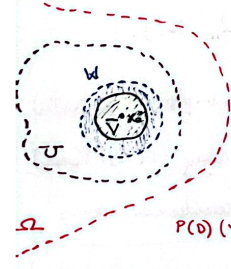
\includegraphics[height=0.3\textheight, width=0.3\textwidth, keepaspectratio]{./Images/24_proof.png}
		\end{center}
	\end{figure}
	Logo,
	\[
		P(D)(\psi u)=\psi f+v,
	\]
	em que \(v\in\mathcal{E}'(U)\) e \(v=0\) em \(W\), pois \(v\) é uma soma de produtos de derivadas \(\partial^{\gamma}\psi\), com \(\gamma\neq0\), por derivadas \(\partial^{\beta}u\), e \(\psi\) é constante em \(W\); além disso,	\(\psi f\in\mathcal{C}_{c}^{\infty}(U).\)

	Por outro lado, das propriedades da convolução e da unicidade obtidas anteriormente, resulta que
	\[
		\psi u
		=E*(\psi f+v)
		=E*(\psi f)+E*v,
	\]
	sendo
	\[
		E*(\psi f)\in\mathcal{C}^{\infty}(\mathbb{R}^{n}).
	\]
	Como \(\psi u=u\) em \(W\), resta provar que \(E*v\) é \(\mathcal{C}^{\infty}\) em alguma vizinhança de \(x_{0}\). É neste ponto que usaremos a hipótese
	\[
		E\in\mathcal{C}^{\infty}(\mathbb{R}^{n}\setminus\{0\}).
	\]

	Para cada \(\varepsilon>0\), consideremos
	\[
		h_{\varepsilon}\in\mathcal{C}_{c}^{\infty}(\overline{B}(0;\varepsilon))
	\]
	com
	\[
		h_{\varepsilon}\equiv1
		\quad\text{em }\overline{B}(0;\varepsilon/2),
	\]	isto é, \(h_{\varepsilon}(x)=1\) quando \(|x|\leq\varepsilon/2\), e escrevamos
	\[
		E=(1-h_{\varepsilon})E+h_{\varepsilon}E.
	\]
	Então
	\[
		E*v=[(1-h_{\varepsilon})E]*v+[(h_{\varepsilon}E)*v].
	\]
	Notemos que
	\[
		(1-h_{\varepsilon})E\in\mathcal{C}^{\infty}(\mathbb{R}^{n}),
	\]
	pois o fator \(1-h_{\varepsilon}\) corta a singularidade de \(E\) na origem. Logo,
	\[
		[(1-h_{\varepsilon})E]*v\in\mathcal{C}^{\infty}(\mathbb{R}^{n}).
	\]

	Observemos ainda que
	\begin{align*}
		\mathrm{supp}[(h_{\varepsilon}E)*v]
		 & \subseteq \mathrm{supp}(h_{\varepsilon}E)+\mathrm{supp}(v) \\
		 & \subseteq \overline{B}(0;\varepsilon)+\mathrm{supp}(v)
		=\overline{\mathcal{O}_{\varepsilon}(\mathrm{supp}(v))},
	\end{align*}
	no qual
	\[
		\mathrm{supp}(v)\cap\overline{V}=\emptyset
	\]
	e, como \(\overline{V}\) e \(\mathrm{supp}(v)\) são compactos disjuntos, existe \(\varepsilon_{0}>0\) tal que, para todo \(0<\varepsilon<\varepsilon_{0}\),
	\[
		\overline{V}\subseteq
		\mathbb{R}^{n}\setminus\mathrm{supp}[(h_{\varepsilon}E)*v].
	\]
	Dessa forma,
	\[
		\mathrm{supp}[(h_{\varepsilon}E)*v]\cap\overline{V}=\emptyset,
	\]
	donde
	\[
		(h_{\varepsilon}E)*v=0
		\quad\text{em }V.
	\]

	Assim,
	\[
		E*v=[(1-h_{\varepsilon})E]*v
		\quad\text{em }V,
	\]
	e, consequentemente, em \(V\) temos
	\[
		u=\psi u
		=\left.E*(\psi f)\right|_{V}
		+\left.[(1-h_{\varepsilon})E]*v\right|_{V}
		\in\mathcal{C}^{\infty}(V).
	\]
	Como \(x_{0}\in U\) foi arbitrário,
	\[
		u\in\mathcal{C}^{\infty}(U),
	\]
	completando a prova. \qedsymbol
\end{proof*}

\end{document}
